\newcounter{espPins}
\def\espWidth{4}
\def\espHeight{8.6}
\def\espScrewThickness{0.125}
\def\espPinHoleThickness{0.07}
\def\espButtonThickness{0.1}

\ctikzsubcircuitdef{spicesp}{
    en, vp, vn, d34, d35, d32, d33, d25, d26, d27, d14, d12, d13, gnd, vin,
    d23, d22, tx0, rx0, d21, d19, d18, d5, tx2, rx2, d4, d2, d15, gnd, 3v3%
} {
    coordinate (#1-origin)
    ++(2,-4.3)
    node (#1) [inner sep = 0pt, anchor = center] {
        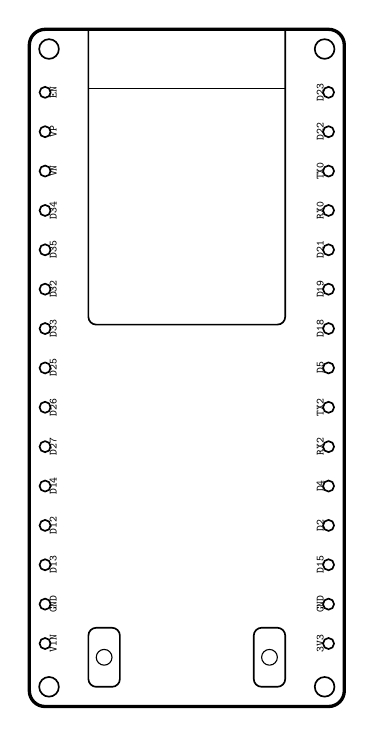
\begin{tikzpicture}
            \setcounter{espPins}{0}
            \draw [rounded corners = 2mm, very thick]
            (0,0) coordinate (origin)
            (origin) rectangle ++(\espWidth,-\espHeight)
            ;
            \draw [semithick] (origin) ++(0.25,-0.25) circle (\espScrewThickness) ;
            \draw [semithick] (origin) ++(\espWidth,0) ++(-0.25,-0.25) circle (\espScrewThickness) ;
            \draw [semithick] (origin) ++(0,-\espHeight) ++(0.25,0.25) circle (\espScrewThickness) ;
            \draw [semithick] (origin) ++(\espWidth,-\espHeight) ++(-0.25,0.25) circle (\espScrewThickness) ;
            %% \foreach \x in {0.8,1.4,...,9.2} {
            %%     \draw (origin) ++(0.25,-\x) circle (0.07);
            %%     \draw (origin) ++(3.75,-\x) circle (0.07);
            %% }
            %% Drawing left pins
            \foreach \x/\y in {0.8/EN, 1.3/VP, 1.8/VN, 2.3/D34, 2.8/D35, 3.3/D32, 3.8/D33, 4.3/D25, 4.8/D26, 5.3/D27, 5.8/D14, 6.3/D12, 6.8/D13, 7.3/GND, 7.8/VIN} {
                \draw [semithick]
                (origin) ++(0.2,-\x) circle (\espPinHoleThickness)
                ++(0.25,0) node [
                    rotate = 90, above = 0pt, font = \tiny, scale = 0.8
                ]{\texttt{\y}}
                ;
            }
            %% Drawing right pins
            \foreach \x/\y in {0.8/D23, 1.3/D22, 1.8/TX0, 2.3/RX0, 2.8/D21, 3.3/D19, 3.8/D18, 4.3/D5, 4.8/TX2, 5.3/RX2, 5.8/D4, 6.3/D2, 6.8/D15, 7.3/GND, 7.8/3V3} {
                \draw [semithick]
                (origin) ++(\espWidth,-\x) ++(-0.2,0) circle (\espPinHoleThickness)
                ++(-0.25,0) node [
                    rotate = 90, below = 0pt, font = \tiny, scale = 0.8
                ]{\texttt{\y}}
                ;
            }
            %% \foreach \x in {}
            %% \begin{scope} [rotate = 90, scale = 0.5, transform shape]
            %%     \draw [white]
            %%     (some)
            %%     coordinate (leftlabel-vrt)
            %%     ++(0.5,-0.5) node [inner sep = 0pt, anchor = north, font = \small] {
            %%         \textbf{VIN}
            %%     }
            %%     ;
            %% \end{scope}
            %% esp
            \draw [semithick, rounded corners = 1mm]
            (origin)
            ++(0.75,0) -- ++(0,-3.75) -- ++(2.5,0) -- ++(0,3.75)
            ;
            \draw [thin]
            (origin)
            ++(0.75,-0.75) -- ++(2.5,0)
            ;
            %% Drawing the buttons
            \draw [semithick, rounded corners = 1mm]
            (origin)
            ++(0.75,-\espHeight)
            ++(0,1) rectangle ++(0.4,-0.75)
            ++(-0.2,0.375) coordinate (enbutton)
            ;
            \draw [thin]
            (enbutton) circle (\espButtonThickness)
            ;
            \draw [semithick, rounded corners = 1mm]
            (origin)
            ++(\espWidth,-\espHeight)
            ++(-0.75,0)
            ++(0,1) rectangle ++(-0.4,-0.75)
            ++(0.2,0.375) coordinate (rstbutton)
            ;
            \draw [thin]
            (rstbutton) circle (\espButtonThickness)
            ;
        \end{tikzpicture}
    }
    %% marking the left pins
    (#1-origin) ++(0,-0.8) coordinate (#1-en)
    (#1-origin) ++(0,-1.3) coordinate (#1-vp)
    (#1-origin) ++(0,-1.8) coordinate (#1-vn)
    (#1-origin) ++(0,-2.3) coordinate (#1-d34)
    (#1-origin) ++(0,-2.8) coordinate (#1-d35)
    (#1-origin) ++(0,-3.3) coordinate (#1-d32)
    (#1-origin) ++(0,-3.8) coordinate (#1-d33)
    (#1-origin) ++(0,-4.3) coordinate (#1-d25)
    (#1-origin) ++(0,-4.8) coordinate (#1-d26)
    (#1-origin) ++(0,-5.3) coordinate (#1-d27)
    (#1-origin) ++(0,-5.8) coordinate (#1-d14)
    (#1-origin) ++(0,-6.3) coordinate (#1-d12)
    (#1-origin) ++(0,-6.8) coordinate (#1-d13)
    (#1-origin) ++(0,-7.3) coordinate (#1-gnd)
    (#1-origin) ++(0,-7.8) coordinate (#1-vin)
    %% marking right pins
    (#1-origin) ++(\espWidth,-0.8) coordinate (#1-d23)
    (#1-origin) ++(\espWidth,-1.3) coordinate (#1-d22)
    (#1-origin) ++(\espWidth,-1.8) coordinate (#1-tx0)
    (#1-origin) ++(\espWidth,-2.3) coordinate (#1-rx0)
    (#1-origin) ++(\espWidth,-2.8) coordinate (#1-d21)
    (#1-origin) ++(\espWidth,-3.3) coordinate (#1-d19)
    (#1-origin) ++(\espWidth,-3.8) coordinate (#1-d18)
    (#1-origin) ++(\espWidth,-4.3) coordinate (#1-d5)
    (#1-origin) ++(\espWidth,-4.8) coordinate (#1-tx2)
    (#1-origin) ++(\espWidth,-5.3) coordinate (#1-rx2)
    (#1-origin) ++(\espWidth,-5.8) coordinate (#1-d4)
    (#1-origin) ++(\espWidth,-6.3) coordinate (#1-d2)
    (#1-origin) ++(\espWidth,-6.8) coordinate (#1-d15)
    (#1-origin) ++(\espWidth,-7.3) coordinate (#1-gnd)
    (#1-origin) ++(\espWidth,-7.8) coordinate (#1-3v3)
}

\ctikzsubcircuitactivate{spicesp}
